\documentclass[a4paper,12pt]{article}
\usepackage{color}
\usepackage{graphicx, gensymb}
\usepackage{amsfonts, cancel, amssymb}
\usepackage{amsmath, amsthm, array, esvect, esint}
\usepackage{typearea}
\usepackage[a4paper,left=2cm,right=2cm,top=2cm,bottom=3cm,bindingoffset=5mm]{geometry}
\usepackage{tikz} 
\usetikzlibrary{shapes,arrows,positioning,automata,backgrounds,calc,er,patterns}
\usepackage{tikz-feynman}
\tikzfeynmanset{compat=1.0.0}
\newcommand\numberthis{\addtocounter{equation}{1}\tag{\theequation}}
\newcommand{\bra}{}
\newcommand{\kom}{}
\newcommand{\brak}{}
\newcommand{\braket}{}
\newcommand{\intx}{}
\newcommand{\intr}{}
\newcommand{\kla}{}
\newcommand{\klam}{}
\newcommand{\klammer}{}
\newcommand{\oper}{}
\newcommand{\tecxt}{}
\newcommand{\Bra}{}
\newcommand{\Ket}{}

\begin{document}

\title{09 Feynman-Regeln}
\author{Joachim Schwardt}
\date{\today}
\maketitle

\section*{Aufgabe 9.1: Lorentz-invarianter Flussfaktor}
Der Flussfaktor ist definiert als $F:=4E_aE_b(|\vec{\beta}_a|+|\vec{\beta}_b|)$. Im Ruhesystem von $b$ gilt $p_b'=(m_b,0)^\top$, und somit $p_a\cdot p_b=p_a'\cdot p_b'=E_a'm_b$. Also gilt:
\begin{align*}
\sqrt{(p_a\cdot p_b)^2-m_a^2m_b^2}=\sqrt{(E_a'm_b)^2-(m_am_b)^2}=m_b|\vec{p}_a\,'|=m_am_b\gamma_a'\beta_a'
\end{align*}
Die relativistische Geschwindigkeitsaddition liefert dabei $\beta_a'=\frac{\beta_a+\beta_b}{1+\beta_a\beta_b}$. Durch Einsetzen erhält man dann das Ergebnis:
\begin{align*}
\gamma_a'\beta_a'&=\frac{\beta_a'}{\sqrt{1-\beta_a'^2}}=\frac{\beta_a + \beta_b}{\sqrt{(1+\beta_a\beta_b)^2-(\beta_a+\beta_b)^2}}=\frac{\beta_a+\beta_b}{\sqrt{1+\beta_a^2\beta_b^2-\beta_a^2-\beta_b^2}}=\\
&=\frac{\beta_a+\beta_b}{\sqrt{(1-\beta_a^2)(1-\beta_b^2)}}=\gamma_a\gamma_b(\beta_a+\beta_b)
\end{align*}
Also gilt die Darstellung $F=4\sqrt{(p_a\cdot p_b)^2-m_a^2m_b^2}$, denn:
\begin{align*}
m_am_b\gamma_a'\beta_a'&=m_am_b\gamma_a\gamma_b(\beta_a+\beta_b)=E_aE_b(|\vec{v}_a|+|\vec{v}_b|)
\end{align*}
\section*{Aufgabe 9.2: 2-2-Streuprozess im Schwerpunktsystem}
Im Schwerpunktsystem gilt $\sum_j\vec{p}_j=0$, also $s=(p_1+p_2)^2=(E_1+E_2)^2$. Die Integration über $\vec{p}_1$ sicher lediglich die Impulserhaltung und kann für die Berechnung zusammen mit der Delta-Distribution weggelassen werden:
\begin{align*}
\sigma &=\frac{(2\pi)^4}{F}\intr\int_{\mathbb{R}^{6}}{|\mathcal{M}_{fi}|^2\delta (E_a+E_b-E_1-E_2)\delta^3(\vec{p}_a+\vec{p}_b-\vec{p}_1-\vec{p}_2)}\,\frac{\mathrm{d}^{3}\vec{p}_1}{(2\pi)^32E_1}\frac{\mathrm{d}^{3}\vec{p}_2}{(2\pi)^32E_2}=\\
&=\frac{1}{(2\pi)^2F}\intr\int_{\mathbb{R}^{3}}{|\mathcal{M}_{fi}|^2\delta (\underbrace{E_a+E_b-E_1-E_2}_{=:f(|\vec{p}_2|)})}\,\frac{\vec{p}_2^2\mathrm{d}^{ }|\vec{p}_2|\mathrm{d}\Omega_2}{4E_1E_2}
\end{align*}
Die einzige Nullstelle von $f=E_a+E_b-\sqrt{m_1^2+\vec{p}_2^2}-\sqrt{m_2^2+\vec{p}_2^2}$ ist beim tatsächlichen Impuls $|\vec{p}_2^{(0)}|$ und es gilt mit $f'=-\frac{|\vec{p}_2|}{E_1}-\frac{|\vec{p}_2|}{E_2}$:
\begin{align*}
\delta(f)&=\frac{\delta(|\vec{p}_2|-|\vec{p}_2^{(0)}|)}{|f'(|\vec{p}_2^{(0)}|)|}=\frac{E_1E_2}{E_1+E_2}\frac{\delta(|\vec{p}_2|-|\vec{p}_2^{(0)}|)}{|\vec{p}_2^{(0)}|}
\end{align*}
Einsetzen vereinfacht den Ausdruck für den Wirkungsquerschnitt, wobei nach der Integration $|\vec{p}_2^{(0)}|\equiv |\vec{p}_f|$ gesetzt wird:
\begin{align*}
\sigma &=\frac{1}{(2\pi)^2F}\intr\int_{\mathbb{R}^{3}}{|\mathcal{M}_{fi}|^2\frac{\delta(|\vec{p}_2|-|\vec{p}_2^{(0)}|)}{|\vec{p}_2^{(0)}|}}\,\frac{|\vec{p}_2|^2\mathrm{d}^{ }|\vec{p}_2|\mathrm{d}\Omega_2}{4(E_1+E_2)}=\\
&=\frac{1}{(2\pi)^2F}\frac{|\vec{p}_f|}{4\sqrt{s}}\oint |\mathcal{M}_{fi}|^2\,\mathrm{d}\Omega
\end{align*}
Im Schwerpunktsystem kann der Flussfaktor mit $\vec{p}_a=-\vec{p}_b$ noch anders ausgedrückt werden, wobei $E_a=\frac{|\vec{p}_a|}{\beta_a}$, $m_a^2=|\vec{p}_a|^2\kla\left( {\frac{1}{\beta_a^2}-1} \right)$ und $m_b^2=|\vec{p}_a|^2\kla\left( {\frac{1}{\beta_b^2}-1} \right)$:
\begin{align*}
F&=4\sqrt{(E_aE_b+\vec{p}_a^2)^2-m_a^2m_b^2}=4\vec{p}_a^2\sqrt{\kla\left( {\frac{1}{\beta_a\beta_b}+1} \right)^2-\kla\left( {\frac{1}{\beta_a^2}-1} \right)^2\kla\left( {\frac{1}{\beta_b^2}-1} \right)}=\\
&=4\vec{p}_a^2\sqrt{\frac{1}{\beta_a^2}+\frac{1}{\beta_b^2}+\frac{2}{\beta_a\beta_b}}=4\vec{p}_a^2\kla\left( {\frac{1}{\beta_a}+\frac{1}{\beta_b}} \right)=4|\vec{p}_a|(E_a+E_b)
\end{align*}
Damit lautet dann das Endergebnis mit $|\vec{p}_{1,2}|\equiv |\vec{p}_i|$:
\begin{align*}
\sigma &=\frac{1}{64\pi^2(E_1+E_2)^2}\frac{|\vec{p}_f|}{|\vec{p}_i|}\oint |\mathcal{M}_{fi}|^2\,\mathrm{d}\Omega
\end{align*}
\section*{Aufgabe 9.3: Matrix-Elemente aus Feynman-Regeln}
Für den Prozess $e^-e^+\longrightarrow e^-e^+$:
\begin{figure}[h!]
\centering
\begin{minipage}{0.4\textwidth}
\centering
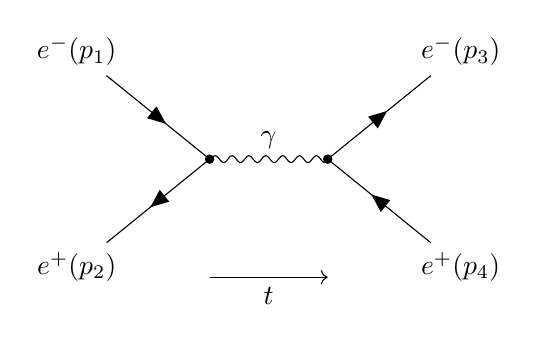
\begin{tikzpicture}
\begin{feynman}
\vertex (a);
\vertex [right=of a] (b);
\vertex [below=of a] (t1);
\vertex [below=of b] (t2);
\vertex [above left=of a] (f1){$e^-(p_1)$};
\vertex [below left=of a] (f2){$e^+(p_2)$};
\vertex [above right=of b] (f3){$e^-(p_3)$};
\vertex [below right=of b] (f4){$e^+(p_4)$};
\diagram*{
(f1) -- [fermion] (a) -- [fermion] (f2),
(a) -- [boson, edge label=$\gamma$] (b),
(f4) -- [fermion] (b) -- [fermion] (f3),
};
\end{feynman}
\draw[->] (t1) -- (t2) node[midway, below] {$t$};
\fill (a) circle (0.06cm);
\fill (b) circle (0.06cm);
\end{tikzpicture}
\caption{s-Kanal}
\end{minipage}
\begin{minipage}{0.4\textwidth}
\centering
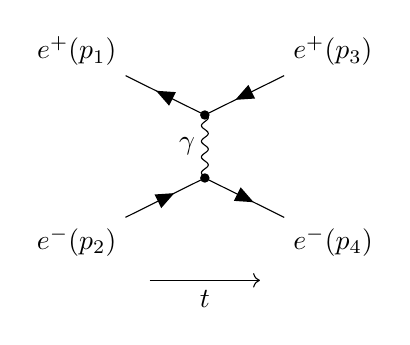
\begin{tikzpicture}
\begin{feynman}
\vertex (a);
\vertex [above=0.8cm of a] (b);
\vertex [below left=1.3cm and 0.7cm of a] (t1);
\vertex [below right=1.3cm and 0.7cm of a] (t2);
\vertex [below right=0.5cm and 1cm of a] (f1){$e^-(p_4)$};
\vertex [below left=0.5cm and 1cm of a] (f2){$e^-(p_2)$};
\vertex [above right=0.5cm and 1cm of b] (f3){$e^+(p_3)$};
\vertex [above left=0.5cm and 1cm of b] (f4){$e^+(p_1)$};
\diagram*{
(f2) -- [fermion] (a) -- [fermion] (f1),
(a) -- [boson, edge label=$\gamma$] (b),
(f3) -- [fermion] (b) -- [fermion] (f4),
};
\end{feynman}
\draw[->] (t1) -- (t2) node[midway, below] {$t$};
\fill (a) circle (0.06cm);
\fill (b) circle (0.06cm);
\end{tikzpicture}
\caption{t-Kanal}
\end{minipage}
\end{figure}\\
Die Mandelstam-Variablen sind $s=(p_1+p_2)^2$, $t=(p_1-p_3)^2$ und $u=(p_1-p_4)^2$:
\begin{align*}
-i\mathcal{M}&=\klam\left[ {\overline{v}(p_2)(-ie\gamma^\mu)u(p_1)} \right]\frac{-ig_{\mu\nu}}{s}\klam\left[ {\overline{u}(p_3)(-ie\gamma^\nu)v(p_4)} \right]
\\
-i\mathcal{M}&=\klam\left[ {\overline{v}(p_1)(-ie\gamma^\mu)v(p_3)} \right]\frac{-ig_{\mu\nu}}{t}\klam\left[ {\overline{u}(p_4)(-ie\gamma^\nu)u(p_2)} \right]
\end{align*}\,\newpage
Für den Prozess $e^-\mu^+\longrightarrow e^-\mu^+$:
\begin{figure}[h!]
\centering
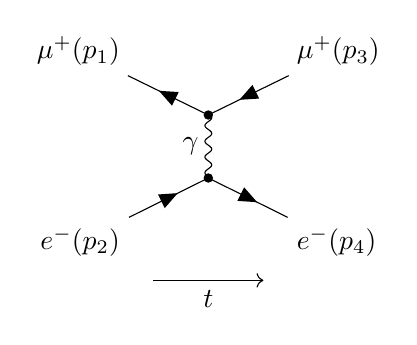
\begin{tikzpicture}
\begin{feynman}
\vertex (a);
\vertex [above=0.8cm of a] (b);
\vertex [below left=1.3cm and 0.7cm of a] (t1);
\vertex [below right=1.3cm and 0.7cm of a] (t2);
\vertex [below right=0.5cm and 1cm of a] (f1){$e^-(p_4)$};
\vertex [below left=0.5cm and 1cm of a] (f2){$e^-(p_2)$};
\vertex [above right=0.5cm and 1cm of b] (f3){$\mu^+(p_3)$};
\vertex [above left=0.5cm and 1cm of b] (f4){$\mu^+(p_1)$};
\diagram*{
(f2) -- [fermion] (a) -- [fermion] (f1),
(a) -- [boson, edge label=$\gamma$] (b),
(f3) -- [fermion] (b) -- [fermion] (f4),
};
\end{feynman}
\draw[->] (t1) -- (t2) node[midway, below] {$t$};
\fill (a) circle (0.06cm);
\fill (b) circle (0.06cm);
\end{tikzpicture}
\caption{t-Kanal}
\end{figure}\\
Hier gilt:
\begin{align*}
-i\mathcal{M}&=\klam\left[ {\overline{v}(p_1)(-ie\gamma^\mu)v(p_3)} \right]\frac{-ig_{\mu\nu}}{t}\klam\left[ {\overline{u}(p_4)(-ie\gamma^\nu)u(p_2)} \right]
\end{align*}
Für den Prozess $e^-e^-\longrightarrow e^-e^-$:
\begin{figure}[h!]
\centering
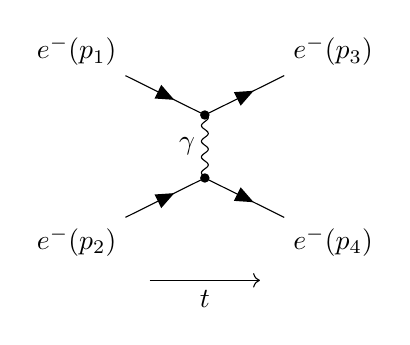
\begin{tikzpicture}
\begin{feynman}
\vertex (a);
\vertex [above=0.8cm of a] (b);
\vertex [below left=1.3cm and 0.7cm of a] (t1);
\vertex [below right=1.3cm and 0.7cm of a] (t2);
\vertex [below right=0.5cm and 1cm of a] (f1){$e^-(p_4)$};
\vertex [below left=0.5cm and 1cm of a] (f2){$e^-(p_2)$};
\vertex [above right=0.5cm and 1cm of b] (f3){$e^-(p_3)$};
\vertex [above left=0.5cm and 1cm of b] (f4){$e^-(p_1)$};
\diagram*{
(f2) -- [fermion] (a) -- [fermion] (f1),
(a) -- [boson, edge label=$\gamma$] (b),
(f4) -- [fermion] (b) -- [fermion] (f3),
};
\end{feynman}
\draw[->] (t1) -- (t2) node[midway, below] {$t$};
\fill (a) circle (0.06cm);
\fill (b) circle (0.06cm);
\end{tikzpicture}
\caption{t-Kanal}
\end{figure}\\
Hier gilt:
\begin{align*}
-i\mathcal{M}&=\klam\left[ {\overline{u}(p_3)(-ie\gamma^\mu)u(p_1)} \right]\frac{-ig_{\mu\nu}}{t}\klam\left[ {\overline{u}(p_4)(-ie\gamma^\nu)u(p_2)} \right]
\end{align*}
Für den Prozess $\gamma\gamma\longrightarrow \gamma\gamma$:
\begin{figure}[h!]
\centering
\begin{minipage}{0.3\textwidth}
\centering
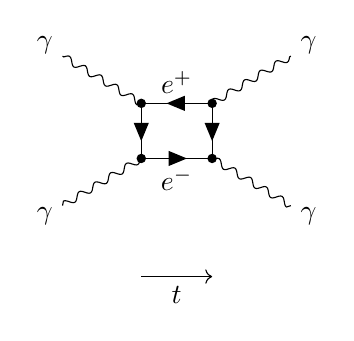
\begin{tikzpicture}
\begin{feynman}
\vertex (a);
\vertex [right=0.9cm of a] (b);
\vertex [above=0.7cm of a] (c);
\vertex [above=0.7cm of b] (d);
\vertex [below=of a] (t1);
\vertex [below=of b] (t2);
\vertex [above left=0.5cm and 1cm of c] (f1){$\gamma$};
\vertex [below left=0.5cm and 1cm of a] (f2){$\gamma$};
\vertex [above right=0.5cm and 1cm of d] (f3){$\gamma$};
\vertex [below right=0.5cm and 1cm of b] (f4){$\gamma$};
\diagram*{
(f1) -- [boson] (c) -- [fermion] (a) -- [boson] (f2),
(a) -- [fermion, edge label'=$e^-$] (b),
(d) -- [fermion, edge label'=$e^+$] (c),
(f3) -- [boson] (d) -- [fermion] (b) -- [boson] (f4),
};
\end{feynman}
\draw[->] (t1) -- (t2) node[midway, below] {$t$};
\fill (a) circle (0.06cm);
\fill (b) circle (0.06cm);
\fill (c) circle (0.06cm);
\fill (d) circle (0.06cm);
\end{tikzpicture}
\end{minipage}
\begin{minipage}{0.3\textwidth}
\centering
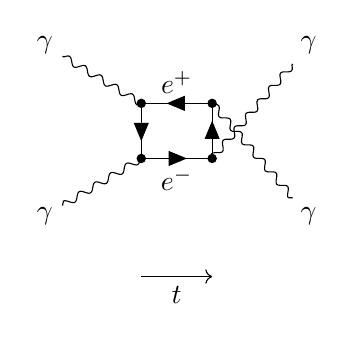
\begin{tikzpicture}
\begin{feynman}
\vertex (a);
\vertex [right=0.9cm of a] (b);
\vertex [above=0.7cm of a] (c);
\vertex [above=0.7cm of b] (d);
\vertex [below=of a] (t1);
\vertex [below=of b] (t2);
\vertex [above left=0.5cm and 1cm of c] (f1){$\gamma$};
\vertex [below left=0.5cm and 1cm of a] (f2){$\gamma$};
\vertex [above right=0.5cm and 1cm of d] (f3){$\gamma$};
\vertex [below right=0.5cm and 1cm of b] (f4){$\gamma$};
\diagram*{
(f1) -- [boson] (c),
(a) -- [boson] (f2),
(a) -- [fermion, edge label'=$e^-$] (b) -- [fermion] (d) -- [fermion, edge label'=$e^+$] (c) -- [fermion] (a),
(f3) -- [boson] (b), 
(d) -- [boson] (f4),
};
\end{feynman}
\draw[->] (t1) -- (t2) node[midway, below] {$t$};
\fill (a) circle (0.06cm);
\fill (b) circle (0.06cm);
\fill (c) circle (0.06cm);
\fill (d) circle (0.06cm);
\end{tikzpicture}
\end{minipage}
\begin{minipage}{0.3\textwidth}
\centering
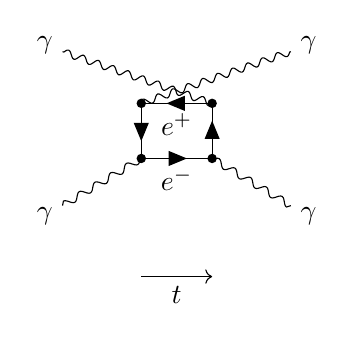
\begin{tikzpicture}
\begin{feynman}
\vertex (a);
\vertex [right=0.9cm of a] (b);
\vertex [above=0.7cm of a] (c);
\vertex [above=0.7cm of b] (d);
\vertex [below=of a] (t1);
\vertex [below=of b] (t2);
\vertex [above left=0.5cm and 1cm of c] (f1){$\gamma$};
\vertex [below left=0.5cm and 1cm of a] (f2){$\gamma$};
\vertex [above right=0.5cm and 1cm of d] (f3){$\gamma$};
\vertex [below right=0.5cm and 1cm of b] (f4){$\gamma$};
\diagram*{
(f1) -- [boson] (d),
(a) -- [boson] (f2),
(a) -- [fermion, edge label'=$e^-$] (b) -- [fermion] (d) -- [fermion, edge label=$e^+$] (c) -- [fermion] (a),
(f3) -- [boson] (c), 
(b) -- [boson] (f4),
};
\end{feynman}
\draw[->] (t1) -- (t2) node[midway, below] {$t$};
\fill (a) circle (0.06cm);
\fill (b) circle (0.06cm);
\fill (c) circle (0.06cm);
\fill (d) circle (0.06cm);
\end{tikzpicture}
\end{minipage}
\end{figure}\\
Hier gilt:
\begin{align*}
-i\mathcal{M}&= (-ie\gamma^\mu\epsilon_\mu (p_1))\frac{-i(\gamma^\kappa (p_1+p_2)_\kappa +m)}{s-m^2} (-ie\gamma^\nu\epsilon_\nu (p_2))\frac{-i(\gamma^\kappa (p_1-p_3)_\kappa +m)}{t-m^2}\\
&\ \ \ (-ie\gamma^\alpha\epsilon_\alpha^\ast (p_3))\frac{-i(\gamma^\kappa (p_2-p_4)_\kappa +m)}{t-m^2}(-ie\gamma^\beta\epsilon_\beta^\ast (p_4))\frac{-i(\gamma^\kappa (p_3+p_4)_\kappa +m)}{s-m^2}
\end{align*}\,\newpage
Für den Prozess $e^-\gamma\longrightarrow e^-\gamma$:
\begin{figure}[h!]
\centering
\begin{minipage}{0.4\textwidth}
\centering
\begin{tikzpicture}
\begin{feynman}
\vertex (a);
\vertex [right=of a] (b);
\vertex [below=of a] (t1);
\vertex [below=of b] (t2);
\vertex [above left=of a] (f1){$\gamma$};
\vertex [below left=of a] (f2){$e^-$};
\vertex [below right=of b] (f3){$\gamma$};
\vertex [above right=of b] (f4){$e^-$};
\diagram*{
(f2) -- [fermion] (a) -- [fermion, edge label=$e^-$] (b) -- [fermion] (f4),
(f1) -- [boson] (a),
(b) -- [boson] (f3),
};
\end{feynman}
\draw[->] (t1) -- (t2) node[midway, below] {$t$};
\fill (a) circle (0.06cm);
\fill (b) circle (0.06cm);
\end{tikzpicture}
\caption{s-Kanal}
\end{minipage}
\begin{minipage}{0.4\textwidth}
\centering
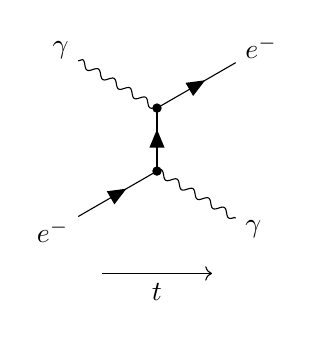
\begin{tikzpicture}
\begin{feynman}
\vertex (a);
\vertex [above=0.8cm of a] (b);
\vertex [below left=1.3cm and 0.7cm of a] (t1);
\vertex [below right=1.3cm and 0.7cm of a] (t2);
\vertex [below right=0.5cm and 1cm of a] (f1){$\gamma$};
\vertex [below left=0.5cm and 1cm of a] (f2){$e^-$};
\vertex [above right=0.5cm and 1cm of b] (f3){$e^-$};
\vertex [above left=0.5cm and 1cm of b] (f4){$\gamma$};
\diagram*{
(f2) -- [fermion] (a) -- [fermion] (b) -- [fermion] (f3),
(f1) -- [boson] (a),
(b) -- [boson] (f4),
};
\end{feynman}
\draw[->] (t1) -- (t2) node[midway, below] {$t$};
\fill (a) circle (0.06cm);
\fill (b) circle (0.06cm);
\end{tikzpicture}
\caption{t-Kanal}
\end{minipage}
\end{figure}\\
Hier gilt:
\begin{align*}
-i\mathcal{M}&=(-ie\gamma^\mu\epsilon_\mu (p_1))\klam\left[ {\overline{u}(p_3)\frac{-i(\gamma^\kappa (p_1+p_2)_\kappa +m)}{s-m^2}u(p_2)} \right](-ie\gamma^\mu\epsilon^\ast_\mu (p_4))\\
-i\mathcal{M}&=(-ie\gamma^\mu\epsilon_\mu (p_1))\klam\left[ {\overline{u}(p_3)\frac{-i(\gamma^\kappa (p_1-p_3)_\kappa +m)}{t-m^2}u(p_2)} \right](-ie\gamma^\mu\epsilon^\ast_\mu (p_4))
\end{align*}
\end{document}